

\tikzset{every picture/.style={line width=0.75pt}} %set default line width to 0.75pt        

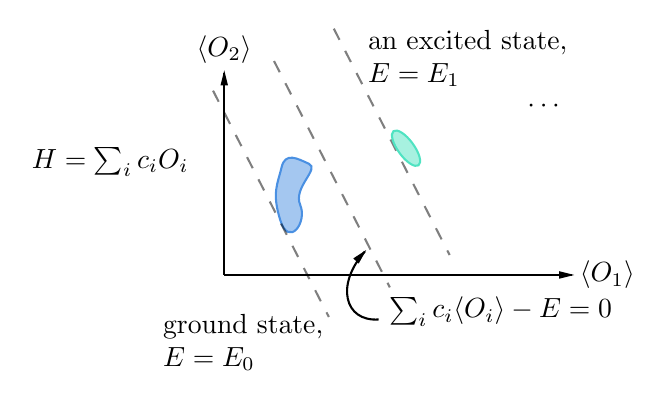
\begin{tikzpicture}[x=0.75pt,y=0.75pt,yscale=-0.6,xscale=0.6]
%uncomment if require: \path (0,353); %set diagram left start at 0, and has height of 353

%Straight Lines [id:da904255078328454] 
\draw    (177,246) -- (456,246) ;
\draw [shift={(458,246)}, rotate = 180] [fill={rgb, 255:red, 0; green, 0; blue, 0 }  ][line width=0.08]  [draw opacity=0] (12,-3) -- (0,0) -- (12,3) -- cycle    ;
%Straight Lines [id:da28860077544833507] 
\draw    (177,246) -- (177,83.73) ;
\draw [shift={(177,81.73)}, rotate = 90] [fill={rgb, 255:red, 0; green, 0; blue, 0 }  ][line width=0.08]  [draw opacity=0] (12,-3) -- (0,0) -- (12,3) -- cycle    ;
%Shape: Polygon Curved [id:ds05129166801576668] 
\draw  [color={rgb, 255:red, 74; green, 144; blue, 226 }  ,draw opacity=1 ][fill={rgb, 255:red, 74; green, 144; blue, 226 }  ,fill opacity=0.5 ] (223,159.73) .. controls (226,146.73) and (236,152.73) .. (245,156.73) .. controls (254,160.73) and (232,175.73) .. (238,189.73) .. controls (244,203.73) and (229,224.27) .. (222,202) .. controls (215,179.73) and (220,172.73) .. (223,159.73) -- cycle ;
%Straight Lines [id:da6483527344854445] 
\draw [color={rgb, 255:red, 0; green, 0; blue, 0 }  ,draw opacity=0.5 ] [dash pattern={on 4.5pt off 4.5pt}]  (168,98) -- (261,279.73) ;
%Straight Lines [id:da0036541181567224523] 
\draw [color={rgb, 255:red, 0; green, 0; blue, 0 }  ,draw opacity=0.5 ] [dash pattern={on 4.5pt off 4.5pt}]  (217,74.27) -- (310,256) ;
%Straight Lines [id:da34767057063343554] 
\draw [color={rgb, 255:red, 0; green, 0; blue, 0 }  ,draw opacity=0.5 ] [dash pattern={on 4.5pt off 4.5pt}]  (265,48.27) -- (358,230) ;
%Shape: Ellipse [id:dp302165402812995] 
\draw  [color={rgb, 255:red, 80; green, 227; blue, 194 }  ,draw opacity=1 ][fill={rgb, 255:red, 80; green, 227; blue, 194 }  ,fill opacity=0.5 ] (312.97,130.5) .. controls (310.07,132.62) and (312.21,140.48) .. (317.75,148.06) .. controls (323.29,155.64) and (330.13,160.08) .. (333.03,157.96) .. controls (335.93,155.84) and (333.79,147.98) .. (328.25,140.4) .. controls (322.71,132.81) and (315.87,128.38) .. (312.97,130.5) -- cycle ;
%Curve Lines [id:da7414078371933952] 
\draw    (301,281.73) .. controls (273.42,283.7) and (266.21,253.65) .. (289.9,227.21) ;
\draw [shift={(291,226)}, rotate = 133.09] [fill={rgb, 255:red, 0; green, 0; blue, 0 }  ][line width=0.08]  [draw opacity=0] (12,-3) -- (0,0) -- (12,3) -- cycle    ;

% Text Node
\draw (460,246) node [anchor=west] [inner sep=0.75pt]    {$\langle O_{1} \rangle $};
% Text Node
\draw (177,78.33) node [anchor=south] [inner sep=0.75pt]    {$\langle O_{2} \rangle $};
% Text Node
\draw (307,261.4) node [anchor=north west][inner sep=0.75pt]    {$\sum _{i} c_{i} \langle O_{i} \rangle -E=0$};
% Text Node
\draw (259,275) node [anchor=north east] [inner sep=0.75pt]   [align=left] {ground state,\\$\displaystyle E=E_{0}$};
% Text Node
\draw (290,97.27) node [anchor=south west] [inner sep=0.75pt]   [align=left] {an excited state,\\$\displaystyle E=E_{1}$};
% Text Node
\draw (418,103.4) node [anchor=north west][inner sep=0.75pt]    {$\cdots $};
% Text Node
\draw (20,141.4) node [anchor=north west][inner sep=0.75pt]    {$H=\sum _{i} c_{i} O_{i}$};


\end{tikzpicture}
